%!TEX root = ../../thesis.tex
\define{\chapterpath}{\allchapterspath/conclusion}
\define{\imgpath}{\chapterpath/img}

\chapter{Conclusion}
\label{chapter:conclusion}
\minitoc

In this thesis, we have developed a set of algorithmic solutions to deal with the problem of \emph{learning from unlabeled interaction frames}. We proposed several methods to exploit the assumption that users are coherent in their teaching behaviors, and to allow the learning agent to improve its performance by actively selecting its next actions.

In this chapter, we summarize our contributions and highlight the most important ideas and algorithm properties of this work. Finally, we explicit a number of possible directions for future research in this domain. We particularly highlight two important directions. The first is to study the property of our problem in a more theoretical way (e.g. convergence properties, effects of world properties). The second direction is the importance of testing this algorithm with a multitude of users in a variety of tasks, we particularly highlight the potential difference between intuitive and adaptive interfaces. As a final note, we highlight the challenge of learning new meanings and identifying new interaction protocols through practical interaction with humans.

%%%%%%%%%%%%%%%%%%%%%%%%%%%%%%%%%%%%%%%%%%%%%%
%%%%%%%%%%%%%%%%%%%%%%%%%%%%%%%%%%%%%%%%%%%%%%
%%%%%%%%%%%%%%%%%%%%%%%%%%%%%%%%%%%%%%%%%%%%%%
%%%%%%%%%%%%%%%%%%%%%%%%%%%%%%%%%%%%%%%%%%%%%%
%%%%%%%%%%%%%%%%%%%%%%%%%%%%%%%%%%%%%%%%%%%%%%
\section{Summary of contributions}

The main objective of this thesis is to endow the interested readers with sufficient understanding of the problem of \emph{learning from unlabeled interaction frames} to implement their own version of the algorithm with the tools they are more familiar with.

Our main contribution is a method allowing a user to start teaching a robot a new task using its own preferred teaching signals. The machine will learn simultaneously which signals are associated to which meaning, as well as identify the task the user wants to solve. Our method consists of generating interpretation hypotheses of the teaching signals with respect to a set of possible tasks. We then assume that the correct task is the one that explains better the history of interaction.

We can highlight four important contributions of this thesis: \begin{inparaenum}[(1)] \item we proposed a new experimental setup to study the co-construction of interaction protocols in collaborative tasks with humans (chapter~\ref{chapter:humanexperiment}); \item we presented an algorithm allowing to simultaneously learn a new task from human instructions as well as the mapping between human instruction signals and their meanings (chapter~\ref{chapter:lfui}); \item we described a measure of uncertainty on the joint task-signal space that takes into account both the uncertainty inherent to the task, as well as the uncertainty about the signal to meaning mapping (chapter~\ref{chapter:planning}); and \item we showed the applicability of the approach to brain-machine interfaces based on error potentials which could work out of the box without calibration, a long-desired property of this type of systems (chapter~\ref{chapter:bci}). \end{inparaenum}

We also proposed a number of possible extensions releasing several assumptions made by our initial algortihm. We address the problems of continuous state space (chapter~\ref{chapter:limitations:continousstate}), continuous task hypothesis space (chapter~\ref{chapter:limitations:continoushypothesis}) and unspecified interaction frames (chapter~\ref{chapter:limitations:framehypothesis}). 

% Our results make us envision the use of our algorithm in more complex scenarios more suited to real world robotics applications.

% This combination allows: 
% \begin{inparaenum}[a)]
% \item a human to start interacting with a system without calibration;
% \item to automatically adapt calibration time to the user needs which can even outperform fixed calibration procedures; 
% \item to adapt to the uncertainty of the information source from scratch.
% \end{inparaenum}

% We showed the applicability of the approach to brain-machine interfaces based on error potentials which could work out of the box without calibration, a long-desired property of this type of systems. 

\paragraph{} We believe the theoretical and empirical work presented in this thesis can constitute an important first step towards flexible personalized teaching interfaces, a key for the future of personal robotics.

%%%%%%%%%%%%%%%%%%%%%%%%%%%%%%%%%%%%%%%%%%%%%%
%%%%%%%%%%%%%%%%%%%%%%%%%%%%%%%%%%%%%%%%%%%%%%
%%%%%%%%%%%%%%%%%%%%%%%%%%%%%%%%%%%%%%%%%%%%%%
%%%%%%%%%%%%%%%%%%%%%%%%%%%%%%%%%%%%%%%%%%%%%%
%%%%%%%%%%%%%%%%%%%%%%%%%%%%%%%%%%%%%%%%%%%%%%
\section{Take home messages: ideas and algorithm properties}

% \section{Main ideas and algorithm properties}

There is three main aspects we would like the reader to take home. First, a source of information does not always apply only on the task space, or on the signal space, but can sometime be observed by combining constraints from both the task and the signal spaces. Secondly, we want to higlight the two operating modes of our algortihm, which first identifies the tasks by measuring the coherence of their signal models and then relies more on an individual classification of signals. Finally, it is important to not feel limited by our examples and to understand that an intercation frame is a generic concept which can be applied to a variety of problems.

% Therefore only the defintion of the problem and the visual example are my main concern the main take home message is that by generating hypothesis about the possible tasks, different interpreationg of the signals emerges among which the more coherent is assumed to be the one taught by the teacher. \todo{look for the formulation of a reviewer}

\subsection{Exploiting information on the joint task-signal space}

Our algorithm relies on measuring the coherence between the spacial organization of the signal and their labels. We link this coherence with the performance of a classifier trained on hypothesized signal-label pairs. This source of information does not provide a direct knowledge about the task, neither about how to decode the signals themselves. It rather provides information emerging from the joint combination of a task and the signals. That is, that for the correct task, the spacial organization of the signal will match with their associated labels. 

This type of information, that acts neither on the task, neither on the signal decoder, but rather on the combination of both is at the core of this work. It has not been often considered in the literature. We highlighted the work of Cederborg et al. (section~\ref{chapter:related:language:thomas}), which make use of a similar source of information reasoning about the consistency of some gestures with respect to different geographical references.

In the BCI community, the work of Kindermans et al. highlights well the use and differences between different information sources \cite{kindermans2014integrating}. They considered a P300 spelling task, and used transfer learning to acquire prior information of the signal decoder. They also used a language model to acquire prior information on the task (i.e. on the possible next letter). And they finally exploit the particular fact that among the multiple stimulations only one event out of six encodes a P300 potential in the speller paradigm. This latter information is a property of the speller paradigm that emerges on the signal space but only for the correct task.

We advocate that this kind of information sources will play an important role in developing flexible personalized teaching interfaces, which can not rely on known information about the task or the signals independently.

\subsection{Two modes}

Our algorithm is divided into a classification algorithm, estimating one classifier for each hypothesis based on past interaction, and a filtering algorithm that uses the predictions and properties of this classifier to update a belief over all tasks hypothesis. The key point is that each hypothesis is considered as if it was the true one. We model the signal to meaning mapping of the user with respect to each task. We then simply test if each classifier can make accurate predictions. As the user is acting according to only one hypothesis, only that hypothesis will be able to predict correctly future interactions. Once a task is identified, we have access to the true intended labels of the user. Which we transfer to all the other hypotheses and start learning a new task using the same equation and by continuing the interpretation hypothesis process. As all hypothesis now share a common set of signal-label pairs, we should be able to learn the new task faster.

We highlight the different processes acting during a full experiment when learning multiple tasks. We will refer to two operating modes: \begin{inparaenum}[a)] \item mode 1 is learning the first task from unlabeled instructions, and \item mode 2 is learning a task when most of the labels are shared between hypothesis. \end{inparaenum} Our update equation is the same for the two operating modes but different properties are more or less active during mode 1 or mode 2.

We remind that our update equation is computed from three terms: 
\begin{itemize}
\item $p(l^f|s,a,\xi)$ is the frame function, it represents the probability distributions of the meanings according to a task, the executed action and the current state, i.e. it represent the interaction frame. 
\item $p(l^c | e, \theta)$ is the raw prediction of the classifier $\theta$. 
\item $p(l^{cc} | l^c, \theta)$ encodes which label should be actually recovered by $\theta$. It is the probability that the classifier itself is reliable in its predictions. 
% Intuitively, it models the quality of the model $\theta$.
\end{itemize}

Mode 1 is the main contribution of this work. During mode 1 is our measure of uncertainty on classifiers' predictions have more impact than the raw predictions of each classifier. Indeed, with very few data available, the classifiers are unable to predict correctly unseen data.
%Even the classifier associated to the correct task is initially of bad quality, due to the noise and dimensionality in the teaching signals. 
Therefore all classifiers are considered as unreliable, and our update equation makes only small updates each step. It is only once one classifier stands apart as being more reliable than the others that differences between likelihoods will emerges. Mode 1 can be observed on Figure~\ref{fig:sequence_evolution} (top), where, during the learning of the first task, all classifier have accuracy close to random (50\%). It is only at step 83 that the correct hypothesis stands apart by being consistently more reliable than the other.

% By doing so the system ends up knowing what is the task taught by the teacher and consequently what are the true labels associated to the teaching signals. Consequently, at the end of phase 1, the system knows a lot more about the mapping between human signals and their meaning.

Mode 2 is almost the contrary. Once many tasks have been identified, all hypothesis share a similar classifier because of the transfer of labels. Therefore they all have similar confusion matrix and make similar predictions. Mode 2 is therefore similar to learning from a known source of information, where all tasks share the same classifier. And it is only by comparing the label prediction of new signals to their expected label for each task that we differentiate hypotheses. This process is logically faster than mode 1 because strong updates are made for each received signal. Mode 2 can be observed on Figure~\ref{fig:sequence_evolution} (top), where, after the step 200, the difference between classifier qualities is very small. Indeed, 5 tasks have already been identified and all hypotheses share most of their signal-label pairs, therefore all classifiers make similar predictions. 

Between mode 1 and mode 2 is a period of transition where the effects of both modes are active. When only few signal-label pairs are shared between hypothesis, each classifier evolve quickly as new observations comes in. This transition can be observed on Figure~\ref{fig:sequence_evolution} (top) between step 83 and 200.

% After the first task is identified, we have access to the true labels associated to each signals but we keep updating all the classifiers. And as the number of shared signal-label pairs is not big enough, 

% In the beginning phase 2, all the classifiers are the same, the difference between hypothesis will be on the match between classified signal and expected label. As we interact with the user, some teaching mistake occurs (\textbf{teaching mistake with respect to the hypothesis considered}) that both create non expected prediction from the classifier and decrease the trust I put into my classifier by mixing labels.

To sum up, the same processes are active in both modes and are captured by the same equation (see Equation~\ref{eq:matchingcrossvalidation}). In mode 1, it is the classifier intrinsic quality that has the most impact. In mode 2, it is the classification of each individual signal that has the most impact. 

% These two modes are captured by the same equation (see Equation~\ref{eq:matchingcrossvalidation}) , which compares predicted and expected labels while taking into account the confidence in the predictions of the classifiers using their respective estimated confusion matrix.

Interestingly, our measure of uncertainty presented in chapter~\ref{chapter:planning} applies indifferently to mode 1 or 2 or during the transition between them. Our uncertainty function combines uncertainty on both signal and task space, when former is known (during mode 2 all hypotheses share the same signal model), the latter becomes the sole source of ambiguity.

\subsection{A frame is a generic function}
\label{chapter:limitations:framegeneric}

An interaction frame is not limited to the straightforward meaning correspondence we assumed (feedback and guidance), it can include various aspects of timing (e.g. teaching delays, asynchronous signals), social cues (e.g. gaze of the user), and do not always requires the robot to know how to perform a task. We provide below some examples of what a frame might includes.

\subsubsection*{A task is not always a fixed target}

In this thesis, we only considered tasks represented as a sparse reward function in a discrete state and action MDP. There is no reason to be limited to this representation of a task, especially to concept of a reaching task, where the agent should reach a specific state. For example task could be an endless repetition of actions such as a robot in an assembly line that should assemble a given object again and again.

Considering the feedback and guidance frame, as soon as the policies associated to each task can be provided to the robot, our algorithm can be applied. We present in Figure~\ref{fig:gridwolrdgenericframes} two examples where policies are easy to define but are not always possible to derive in a simple MDP representation.

The policy of Figure~\ref{fig:gridwolrdgenericframesaround} consists of following the external wall of the grid world in a clockwise direction. Similarly in Figure~\ref{fig:gridwolrdgenericframesaround}, the policy consists of an endless looping trajectory. These policies can not be derived from a state based reward function. They are however rather easy to define by hand or to derive from another representation of the task.

\begin{figure}[!htbp]
\centering
    \begin{subfigure}[b]{0.49\columnwidth}
        \centering
        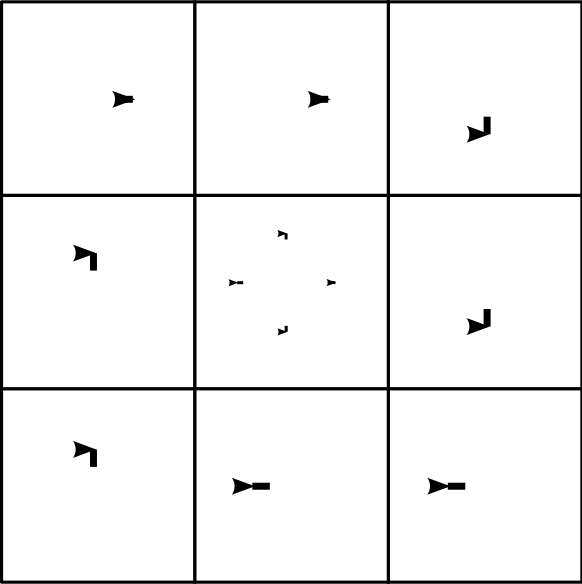
\includegraphics[width=0.6\columnwidth]{\visualspdf/frame/gridworld_around.pdf}
        \caption{}
        \label{fig:gridwolrdgenericframesaround}
    \end{subfigure}
    \begin{subfigure}[b]{0.49\columnwidth}
        \centering
        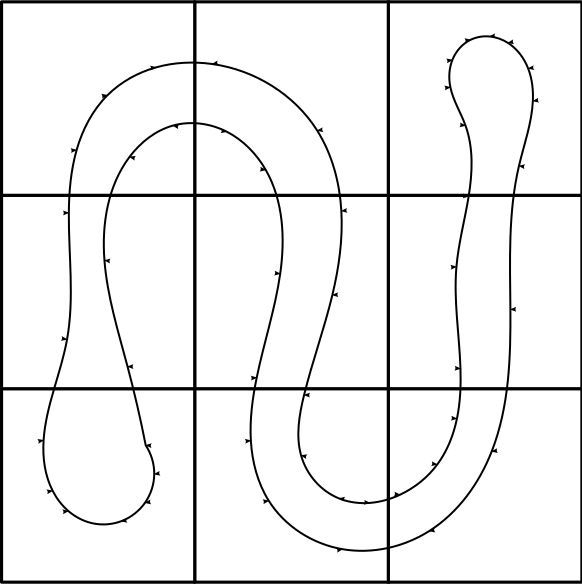
\includegraphics[width=0.6\columnwidth]{\visualspdf/frame/gridworld_loop.pdf}
        \caption{}
        \label{fig:gridwolrdgenericframesloop}
    \end{subfigure}
\caption{Two agent behaviors that are hard to define in terms of reward function.}
\label{fig:gridwolrdgenericframes}
\end{figure}

We note that it is possible, but not always convenient, to represent a problem such that a fixed reward function allows to define the task of Figure~\ref{fig:gridwolrdgenericframesaround}~and~\ref{fig:gridwolrdgenericframesloop}. For Figure~\ref{fig:gridwolrdgenericframesaround} defining a reward function on the state-action space would be enough. For Figure~\ref{fig:gridwolrdgenericframesloop}, it is more challenging as the Markov properties are not respected (we must know the current and previous position of the agent to predict its future position). Therefore the representation of the problem should include the previous position of the agent, which increases the state space from 9 states to 81 states.

\subsubsection*{No need for planning skills}

Although in most of the problem described in this work, the agent needed to know the optimal policy for each task, it is only a specificity of the feedback and guidance frame we considered. For example, in section~\ref{chapter:limitations:continuoushypothesis} we considered a frame where a teacher provides indication about the absolute direction of objects. Therefore, interpreting a signal with respect to various object only requires to know the positions of these objects, without the need to know how to reach each object.

% equiring the robot to be equipped with planning abilities

\subsubsection*{Asynchronous instructions}

The interaction between the user and the machine would be easier if the robot could act continuously and the human could provide instructions when he deemed necessary. Our pick and place scenario of chapter~\ref{chapter:lfui} has been experienced as boring by the users, which had to provide a feedback after each movement of the robot. In some domains, the frequency of actions is to high to afford waiting for a feedback signal between each action. Either the action would be so small that the user would not be able to evaluate it, either the interaction flow and execution time would be dramatically affected by the many pauses in the task execution.

To allow for continuous operation of the robot, asynchronous delivery of signals should be accepted. A potential avenue is to consider a temporal function that distribute a signal event across a subset of previous robot's actions \cite{hockley1984analysis,knox2009interactively}. 

% This method has been used by Knox et al. in their TAMER framework \cite{knox2009interactively} using a data from a study of the distribution of human response times \cite{hockley1984analysis}.

\subsubsection*{Including social clues}

Information known to be true for most interaction scenarios can be included in the frame definition. For example, if the user is looking away from the scene, he is less likely to provide correct feedback. Such information can be included to the frame function by decreasing the probability that the user will provide an appropriate signal if the user is looking away. Other potential sources of teaching mistakes include the presence of other persons in the room, or the fact that some objects are hidden to the teacher's eyes.

% \todo{A frame can be more complex than the simple relation described above. For example, a frame could include the gaze of the user as an indication of the user attention, therefore influencing the probability that the user is making a teaching mistake. For example, if the user is looking away from the scene, he is less likely to provide correct feedback. A frame is also not always related to the actions of the agent, it can be that, when the user show an object to the robot, he also spell the name of that object. This frame allows the robot to learn the name of different objects, this frame is often used in language acquisition experiments (see chapter~\ref{chapter:related:language})}


% In this section, we provide example of what a frames might be. In all the experiment consider until now, we only considered the feedback and guidance frame which implies many constraint on the interaction protocol and the abilities of the robot. For example, the user should deliver feedback after one action of the robot, this simple interaction already requires to implement a turn taking social behavior in the robot, but also means that the user is able to see know when one action has been executed by the robot. On the other side, the robot need to interpret the signal from the user with respect to many objectives, and in our scenarios, this requires the robot to know the optimal plan in each state and for every task hypothesis. 

% This kind of constraints are usual in BCI scenario, where it is still difficult to extract information continuously from ErrP EEG signals and where the task to be execute is often discrete and of low complexity such that it is easy for our agent to compute the optimal policies for each task. 
% In the following of this section we describe a few frame that may be considered for extending this work to more real world robotic scenario.

%%%%%%%%%%%%%%%%%%%%%%%%%%%%%%%%%%%%%%%%%%%%%%
%%%%%%%%%%%%%%%%%%%%%%%%%%%%%%%%%%%%%%%%%%%%%%
%%%%%%%%%%%%%%%%%%%%%%%%%%%%%%%%%%%%%%%%%%%%%%
%%%%%%%%%%%%%%%%%%%%%%%%%%%%%%%%%%%%%%%%%%%%%%
%%%%%%%%%%%%%%%%%%%%%%%%%%%%%%%%%%%%%%%%%%%%%%
\section{Future works}
% \section{Future works in this domain}

The work presented in this thesis opens new perceptive 


% \subsection{Technical challenges}

% remove assumptions such as the one presented is limitation section

\subsection{Theoretical analysis}

The work presented in this thesis mainly focus on empirical experiments. 


such as proof and studies of the properties of the system. 

symmetry cases

By taking inspiration from the proof described in previous chapter, there is many fast imporvmenrt than can be done. Mainly by relaxinfg the assumtion that the user is perfect, or that each task is composed os half optimal and halfp non optimal state action pairs.


\subsection{Target based versus reward maximization scenarios}

as identifued in chapter~\ref{chapter:limitations:wordlproperties}

The main conclusion of our preliminary study is that we do not understand well the impact of some properties of the world and dataset on the final performance of our system. Many of these properties are tightly linked together and the additional layer of uncertainty inherent to our problem makes the dependencies hard to identifies.

However one important aspect highlighted by the study is that our uncertainty measure should be combined with other metrics to optimize additional criteria on the task. 

Our measure was developed to discriminate faster the correct hypothesis from the set of possible tasks and not to also execute that task as fast as possible.



We propose two different types of scenario that are likely to be useful in real world scenario: 
\begin{itemize}
\item Target based scenarios: The goal of the agent is to execute one specific action in a particular state and should not make mistakes in the execution of the task. For example, a robot should put one object to the bin for a human. The robot can navigate around of the objects area in order to collect feedback but should only grasp an object and put it to the bin once it is confident about which object to throw away. This includes all the scenario considered in this thesis, and as seen in this section there is room to improve over our uncertainty method by including information about the hypothesized task. A potential avenue is to merge our measure of uncertainty with the optimal policies for each task, such that, for two states with close uncertainty value, the one closer to the target should be preferred. When all task are equally probable, only the uncertainty should be taken into account. And once there is no more uncertainty, i.e. when confidence is reached, the action should be selected according to the task policy. The main problem is about how to weight the two functions.

\item Reward maximization scenarios: In such scenario the goal of the robot is to maximize the reward associated to the correct task. However, many tasks may share some parts of a reward functions. Therefore it is not always necessary to identify the correct task with confidence to collect maximal rewards. For example, in our puddle word scenario of section~\ref{chapter:limitations:continousstate}, two tasks may share the same goal area but different areas to avoid. If the robot can reach the shared goal area by avoiding both negative areas, then the agent will have maximized the collected reward without ever knowing what specific task the user had in mind. Tackling this problem requires a different approach as the agent should now be confident that merging two reward functions is more optimal than trying to differentiate between them. However the robot can not merge all rewards function right from the start as no specific direction will emerge and the correct reward won't be maximized in the long run.
\end{itemize}

Each of these scenarios requires to develop new exploration method. These challenges remain to be investigate and, if solved, are likely to be of practical interest for real word applications.

\subsection{Applications}

we only considered three domains?

This work opens a new perspective regarding the global challenge of interacting with machines. It has application to many interaction problems which requires a machine to learn how to interpret unknown communicative signals. A promising avenue, outside the BCI field, lies in human robot interaction scenarios where robots must learn from, and interact with, many different users who have their own limitations and preferences.

We hope for the better with application to assistive technologies, but can anticipate the worst, such as customer behavior understanding for advertissing purposes.

\subsection{Studying humans in the loop}
\label{chapter:limitations:userstudies}

\question{Do people want to have an open-ended choice about what signal to use? \\ Would they be more efficient?}

In section~\ref{chapter:limitations:userstudies}, we discuss the need for conducting user studies in more complex domain to evaluate the scalability, efficiency, and acceptability of our method.

Only prerecorded datasets have been used. However, signals may change during the learning. For instance, people can try to adapt themselves to a robot if they believe the latter is not understanding properly. Or, brain signals are sensitive to the protocol, the duration of the experiment or even the percentage of errors made by the agent \cite{chavarriaga2010learning}. To which extend the behavior of our agent changes the properties of the teaching signal? 

Moreover, in real-world applications, users are usually told how to interact with machines. And having a free choice on some details of the interaction may finally become a disadvantage and lower perfomances. Do people want to have an open-ended choice about what signal to use? Would they be more efficient? When is it better to use a calibration procedure?

As we argued in the introduction, the work we presented is a starting point towards forms of adaptive interaction with non-technical users, that we may call fluid interaction learning. While we studied in this thesis properties of learning algorithms that will be needed for such an endeavor, it remains to be shown how they can be integrated within a full real-world human-robot interaction scenario and architecture so that the usability and acceptability of such system can be evaluated. Thus, user studies in particular will be a crucial next step of this work. The improvements described in previous section may be needed to reach acceptable levels of usability.

An interesting direction would be to consider the same experimental setup as the one used in chapter~\ref{chapter:humanexperiment} which allow to seamlessly use a human or a machine on either of the side of the interaction. A natural extension is therefore to replace the human builder by an agent using our algorithm. But one could also study active teaching algorithm \cite{cakmak2012algorithmic}, by replacing the teacher side by an artificial agent.

This kind of experiment would allow to study the same setup with both humans and artificial agents and may open new perspective in both human-robot interaction and experimental semiotic studies. By controlling some aspects of the interaction, on either of the interaction side, one could for example study how the agent behavior affect the teaching behavior of the human. But also study how the teaching behavior of a human influence the understanding and performance of the learner, whether the learner is a human or a machine. 

algorithm assumption on human behavior

discuss how the setup can be used in HRI, but also semiotic stuff...

Users comply with the frame implemented. Same meaning, optimal strategies, timing...

Assumption: The properties of the signals do not change wrt. the behavior of the agent

In relation to targeting fluid interaction learning, we will consider in the future how more complex kinds of instructions can be included in our formalism. Indeed, the possible teaching models used spontaneously by people can be more complex than the simple meaning correspondences we assumed \cite{thomaz2008teachable,Cakmak2010optimality}. Also the turn taking scheme could be made more natural, as the robot could ask questions \cite{cakmak2012designing} and accept asynchronous instructions.

Indeed, our current system can be restrictive for the user as the number of interaction increases quickly with the complexity of the size of the task and meaning spaces. However, we have shown that the system is able to use known sources of information, which in real-world interaction could be leveraged to keep the sample complexity low.

users are not ready maybe, they want intuitive interface, not adaptive.

human exp with a computer at one side, or with some signal not dipslaye,d or with delayed, or with ranodm possition...

cite mohammed chetouanni

\subsection{Creating meanings and interaction protocols}

\question{Who create the frame functions?}

Finally in section~\ref{chapter:limitations:discussion}, we discuss a number of limitations that were not addressed in this work and that are not straightforward to solve given our context. Such as using continuous actions or learning new meanings.

However, to fully address the stated problem of fluid interactive learning, a number of open challenges still remain to be investigated. For example, extending the system towards the creation of novel meanings is an important question, as well as the problem of detecting, and understanding new interaction frames that may allow the user to progressively provide more higher level instructions to the robot. 

A key challenge towards life long learning also lies in dynamic and hierarchical learning architecture, such as for example learning new macro-states and new macro-actions, associated to new macro-instructions.

all this is very high level

learning the meaning is the natural next step, where very few work jave tackled it

how to learn the interaction hypothesis and interaction frame is a big problem, refer to thomas thesis.

coupled with a system that creates the frame, not neccessarily the meaning but at least generate some human behaviors.


The transition from raw input to higher level meaning is however not much investigated in science. Here our agent or robot already have the ability to categorize state, make plans and select what is relevant from the environment.

